\chapter{Mechanized Logic}
\label{ch:mechanized-logic}
%%\begin{comment}

Proofs of algebraic equations
like those in Chapter~\ref{ch:mathematical-induction}
depend on matching grammatical elements in formulas
against templates in axioms and theorems.
A proof starts with a formula on one side
of the equation of a theorem,
cites a known equation to transform the formula
to another one with the same meaning,
and moves gradually, step by step, to the formula
on the other side of the equation of the theorem.
It is easy for people to make mistakes in this detailed, syntax-matching process,
but computers can carry it out flawlessly and
relieve us from an obligation to focus with monk-like devotion on grammatical details.

\begin{aside}
One of the aims of this book is to help students learn to
verify, using rigorous logic, properties of software
that is specified in the form of inductive equations.
Another goal is to provide
an inkling of how a mechanized logic
can formalize reasoning of that kind
and lead to greater confidence in the results.
If you follow the broad outlines of the examples
and successfully work your way through some of the exercises,
we think you will gain a basic understanding
of what can be done with mechanized logic.
Acquiring expertise with such tools
would require substantially more study and experience.
\caption{ACL2 Learning Objectives}
\label{aside:acl2-learning-objectives}
\end{aside}

ACL2 is one of several systems of \index{mechanized logic}\index{logic!mechanized}mechanized logic that provide this
kind of assistance with proofs.
Theorems for the ACL2 proof engine take the same form
as properties for the doublecheck testing facility in Proof Pad.
ACL2 has a built-in way to look for inductive proofs,
and for some theorems it succeeds without guidance.
Most of the time, however, ACL2 needs some help in
finding its way through the morass of strategies.
In any case ACL2 checks the details automatically.

To illustrate how this works, we return to the theorems
discussed in Chapter~\ref{ch:mathematical-induction}.
The syntax of ACL2 requires prefix notation exclusively,
as you would expect, and there are additional issues
to be discussed, but the form of the theorems
will be familiar from your experience with doublecheck.

\section{ACL2 Theorems and Proofs}
\label{sec:theorems-and-acl2-proofs}

The first proof by mathematical induction
in Chapter~\ref{ch:mathematical-induction}
verified the additive law of concatenation
(page \pageref{additive-law-concatenation}).
The statement of the theorem asserted that a proposition L($n$) is true,
regardless of which natural number $n$ stands for: ($\forall$$n$.L($n$)),
where L($n$) stands for the following equation.
\label{eq:Ln-additive-law}
\begin{center}
L($n$) $\equiv$ (len (append [$x_1$ $x_2$ \dots $x_n$] $ys$)) $=$ ($+$ (len [$x_1$ $x_2$ \dots $x_n$]) (len $ys$))
\end{center}

In Chapter~\ref{ch:software-testing-prefix-notation} (page \pageref{additive-lengths-test})
we defined a doublecheck test of this equation.

\begin{Verbatim}
(defproperty additive-law-of-concatenation-test
    (xs :value (random-list-of (random-natural))
     ys :value (random-list-of (random-natural)))
  (= (len (append xs ys))
     (+ (len xs) (len ys))))
\end{Verbatim}

\begin{aside}
\begin{center}
 \setlength{\tabcolsep}{0pt}
\begin{tabular}{ll}
~&L($n$) $\equiv$ (len (append [$x_1$ $x_2$ \dots $x_n$] $ys$)) $=$ ($+$ (len [$x_1$ $x_2$ \dots $x_n$]) (len $ys$))\\
~&~~~versus A($xs$, $ys$) $\equiv$ (len (append $xs$ $ys$)) $=$ ($+$ (len $xs$) (len $ys$))\\
\end{tabular}
\end{center}
\vspace{2mm}
A proof of ($\forall$$n$.L($n$))
is intended to apply to all lists with $n$ elements,
regardless of what those elements are.
The formula $(\forall xs.(\forall ys.$A($xs$, $ys$)$))$
is a more formal statement of the intended theorem,
where A is a predicate whose universe of discourse
is pairs of lists.

A proof of ($\forall$$n$.L($n$)) accomplishes this goal
rigorously (but not with full formality)
if it avoids depending in any way on the elements in the lists that
[$x_1$ $x_2$ \dots $x_n$] and $ys$ stand for, other than
the requirement that $n$ is a natural number.
Furthermore, the proof assumes that any list of length $n$
has a representation in the form [$x_1$ $x_2$ \dots $x_n$].

The \{\emph{lst}\} axiom states this assumption in terms of
the bound variables $xs$ and $n$,
with lists and natural numbers, respectively, as their
universes of discourse and where
[$x_1$ $x_2$ \dots $x_n$] stands for a list of $n$
elements from specifiable domains.
\begin{center}
  Axiom \{\emph{lst}\}: $(\forall xs.(\exists n.(\exists$[$x_1$ $x_2$ \dots $x_n$]$.(xs = $[$x_1$ $x_2$ \dots $x_n$]$))))$
\end{center}
\caption{An Informality: [$x_1$ $x_2$ \dots $x_n$] versus $xs$}
\label{axiom:lst}
\end{aside}

Of course, the doublecheck specification
cannot employ the informal notation of numbered lists
(page \pageref{numbered-list-interpretation}).
Instead, the property uses the variable $xs$ to designate the list.
The ACL2 statement of the theorem corresponding to this property
is the same as the property specification
except for and the keyword ``defproperty'',
which becomes ``defthm,'' and
the random data generators (introduced
by the ``:value'' keyword), which are not present in the theorem.
Theorem statements in ACL2 start with the
\index{defthm}\index{definition!theorem, ACL2}``defthm'' keyword.
After that comes a name for the theorem and the Boolean formula
that states the theorem.

\begin{Verbatim}
(defthm additive-law-of-concatenation-thm
  (= (len (append xs ys))
     (+ (len xs) (len ys))))
\end{Verbatim}

\begin{figure}
\begin{center}
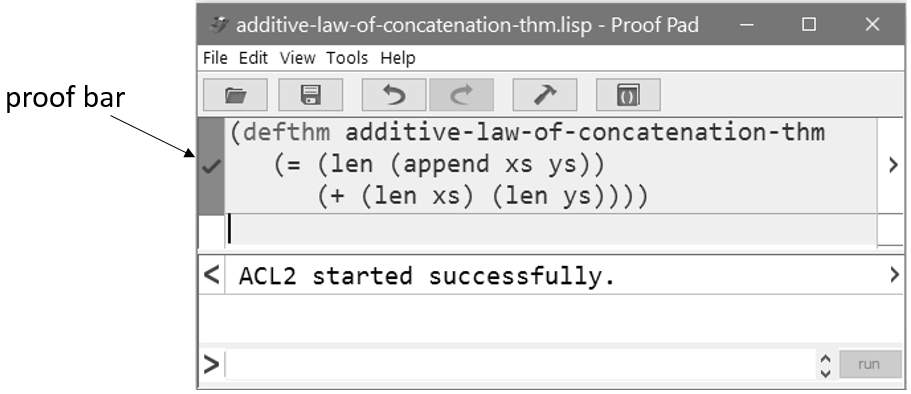
\includegraphics[scale=0.55]{images/additive-law-of-concatenation-thm-acl2-prf-bw.png}
\end{center}
\index{Proof Pad!proof bar}\index{proof bar}
\caption{Proof Pad Session with Proof Bar}
\label{fig:proof-bar-with-chk}
\end{figure}

The mechanized logic of ACL2 fully automates the proof of this theorem.
It follows its own heuristic procedures to find an induction scheme
and pushes the proof through on its own.
To see ACL2 in action, enter the theorem into a Proof Pad session
and click in the green proof bar
(Figure~\ref{fig:proof-bar-with-chk}, page \pageref{fig:proof-bar-with-chk}).
This sets ACL2 in motion to prove the theorem.
A check mark appears in the proof bar
when the mechanized logic succeeds.

\section{Using Books of Proven Theorems}
\label{sec:using-books-of-proven-theorems}

The append-suffix theorem, which states that
if the first operand of the append operator is a list of length $n$,
then dropping $n$ elements from the front of the concatenation
reproduces the second operand of append.
In Section~\ref{sec:append-prefix-suffix} (page \pageref{append-suffix-thm-pencil-proof})
we stated this theorem in the form ($\forall$$n$.S($n$)),
where S($n$) is a shorthand for the following equation.

\begin{samepage}
\begin{center}
S($n$) $\equiv$ (nthcdr (len [$x_1$ $x_2$ \dots $x_n$]) (append [$x_1$ $x_2$ \dots $x_n$] $ys$)) $=$ $ys$
\end{center}
\end{samepage}

In ACL2 notation, a definition of this theorem takes the following form.

\index{append!suffix theorem}\index{theorem!append-suffix}
\index{theorem, by name!\{append-suffix\}}
\begin{Verbatim}
(defthm append-suffix-thm
  (equal (nthcdr (len xs) (append xs ys))
         ys))
\end{Verbatim}

The mechanized logic can prove this theorem, but
the proof depends on some equations from numeric algebra.
Fortunately, ACL2 experts have already proved many such theorems,
and the ACL2 system makes them available in the form of
\index{book!ACL2}\seeonlyindex{ACL2 book}{book}
\index{book!certified}\seeonlyindex{certified book}{book}``certified books''
(ACL2 terminology for a package of theorems successfully proven by the
mechanized logic).
A book known as
\index{book!arithmetic-3/top}
\label{arith-top-book} "arithmetic-3/top"
contains theorems from algebra
\index{theorem!algebra, ACL2}
that the mechanized logic can cite in
a proof of the append-suffix theorem.
An include-book directive tells ACL2
to import these theorems.
\index{directive!include-book}
\index{directory (:dir)!:system}\index{system, :dir}\index{book!directory (:dir)}
\begin{center}
(include-book "arithmetic-3/top" :dir :system)
\end{center}

To make the theorems in the book available
for ACL2 to cite in a proof,
the directive precedes the defthm command that
defines the theorem to be proved, as shown in
Figure~\ref{fig:append-suffix-acl2-prf} (page \pageref{fig:append-suffix-acl2-prf}).
Clicking in the proof bar sets the mechanized logic in motion,
and a check mark appears in the proof bar when
the proof is complete.
To try it for yourself in a Proof Pad session.
Enter the include-book directive
and theorem definition of Figure~\ref{fig:append-suffix-acl2-prf},
click in the proof bar, and see what happens.

\begin{figure}
\begin{center}
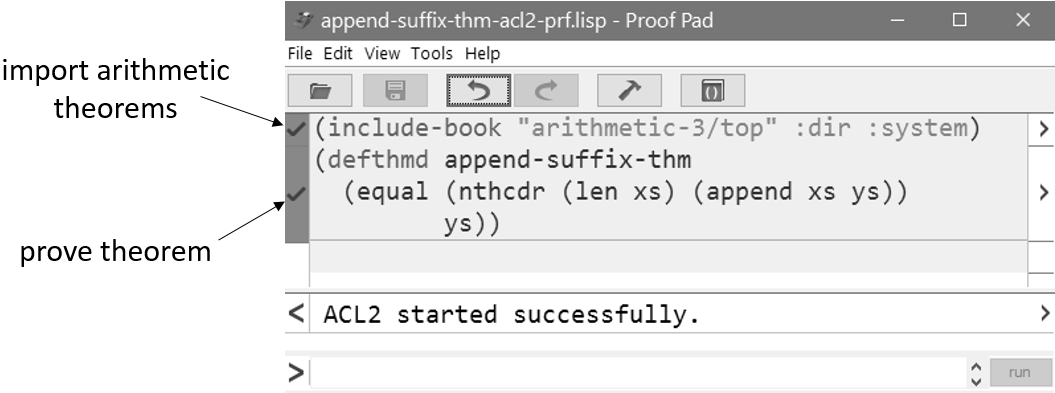
\includegraphics[scale=0.5]{images/append-suffix-thm-acl2-prf-bw.png}
\end{center}
\index{theorem!append-suffix}\index{theorem, by name!\{append-suffix\}}
\index{append!suffix theorem}
\caption{Append-Suffix: Importing Theorems to Cite in Proof}
\label{fig:append-suffix-acl2-prf}
\end{figure}

\begin{ExerciseList}

\Exercise Define the
\index{append!associative}
\index{theorem!append associative}
\index{theorem, by name!\{append associative\}}
\index{associative}\{\emph{append associativity}\}
theorem in ACL2 notation,
and use Proof Pad to run it through the ACL2 mechanized logic.
If you state the theorem correctly, ACL2 will succeed in proving it.\footnote{According
to \index{Moore, J Strother}J Strother Moore, a pioneer
in mechanized logic and a principal developer of ACL2,
the associativity of append was one of the driving examples in early work in
mechanized logic and one of the first theorems that such a system proved autonomously.}

\Exercise Define the following theorem for ACL2 and get the mechanized logic to prove it:
$\forall xs.$((len (nthcdr (len xs) xs)) $=$ 0).

\end{ExerciseList}

\section{Theorems with Constraints}
\label{sec:implies-constraints}

Another of the pencil-and-paper proofs in Section~\ref{sec:append-prefix-suffix}
was the append-prefix theorem
(Figure~\ref{numbered-list-interpretation}, page \pageref{numbered-list-interpretation}),
which referred to the prefix operator.

\begin{Verbatim}
(defun prefix (n xs)
   (if (and (posp n) (consp xs))
       (cons (first xs) (prefix (- n 1) (rest xs))) ; {pfx1}
       nil))                                        ; {pfx0}
\end{Verbatim}

The append-prefix theorem, as stated for the pencil-and-paper proof,
had the form $\forall n.$S$(n)$,
where S($n$)
was written in terms of a numbered list.
The same theorem in ACL2 terminology uses a variable to designate the list.
\begin{samepage}
\begin{quote}
Theorem \{append-prefix\} $\forall n.$S$(n)$ \\
S($n$) $\equiv$ (nthcdr (len [$x_1$ $x_2$ \dots $x_n$]) (append [$x_1$ $x_2$ \dots $x_n$] $ys$)) $=$ $ys$
\begin{Verbatim}
(defthm append-prefix-thm-NOT-QUITE-RIGHT
  (equal (prefix (len xs) (append xs ys))
         xs))
\end{Verbatim}
\end{quote}
\end{samepage}

However, the theorem as stated
is not quite correct,
and to explain why, we need to mention
some things we haven't told you about lists.
\label{true-list-def}
A \emph{true list} in ACL2 is either nil (the empty list)
or a value of the form (cons $x$ $xs$),
where $xs$ is a true list.
It can be verified by induction that
the prefix operator always delivers a true list.
The value (prefix 0 xs) is nil (a true list by definition).
That takes care of the base case.
The value of (prefix $(n+1)$ xs) is either nil (again a true list)
or (cons (first xs) (prefix $n$ (rest xs))).
We can assume by the induction hypothesis that
(prefix $n$ (rest xs)) is a true list,
which means (by the definition of ``true list'')
that (cons (first xs) (prefix $n$ (rest $xs$))) is a true list.
That takes care of the inductive case and completes the proof
that (prefix $n$ $x$s) is always a true list.

When the second operand of cons is not a true list,
the value it constructs isn't a true list, either.
For example, (cons 2 1) is not a true list because 1 is not a true list.
The formula (cons 3 (cons 2 1)) also is not a true list,
again because the second operand,
in this case (cons 2 1), is not a true list.
However, (len (cons 3 (cons 2 1)) is 2, which you can work
out from the axioms or, easier,
just submit the formula to ACL2 and let it do the computation.
A similar computation reveals that
(prefix (len (cons 3 (cons 1 2))) (cons 3 (cons 1 2)))
is (cons 3 (cons 2 nil)), not (cons 3 (cons 2 1)).
That is, when $xs$ is (cons 3 (cons 2 1)),
then (prefix (len xs) (append xs ys)) is not equal to $xs$.
The equation that theorem append-prefix-thm-NOT-QUITE-RIGHT
guarantees does not hold when $xs$ is (cons 3 (cons 2 1)).
Since a theorem cannot have exceptions,
the theorem append-prefix-thm-NOT-QUITE-RIGHT
isn't true.

\begin{aside}
A theorem that takes the form of an implication, $x \rightarrow y$,
says that the conclusion, $y$, will be true when the hypothesis, $x$,
is true, but says nothing about the status of the conclusion when
the hypothesis is false. The ACL2 equivalent of the Boolean formula $x \rightarrow y$
is (implies $x$ $y$).
For example, one can conclude that $u - 1 < v - 1$
if one knows that $u < v$.
In ACL2 this fact would be stated as an implication.
\begin{Verbatim}
(defthm simple-theorem-about-numbers
  (implies (< u v)
           (< (- u 1) (- v 1))))
\end{Verbatim}
\index{theorem!constraints}\index{theorem!implication, constraint}
\caption{Using Implication to Constrain the Domain of a Theorem}
\label{thm-with-implies}
\end{aside}

The theorem is true, however, when the variable $xs$ is
constrained to the domain of true lists.
In the statement of the append-prefix theorem in
Section~\ref{sec:append-prefix-suffix} (page \pageref{append-prefix-thm-predicate}),
the role of $xs$ was played by the numbered list
[$x_1$ $x_2$ \dots $x_n$], which is a true list, by definition
(page \pageref{numbered-list-interpretation}).
ACL2 does not permit the use of the numbered list syntax,
so the true-list constraint must be explicit.
An implication formula imposes the necessary constraint.

\begin{Verbatim}
(defthm append-prefix-thm
   (implies (true-listp xs)
            (equal (prefix (len xs) (append xs ys))
                   xs)))
\end{Verbatim}

\begin{figure}
\begin{center}
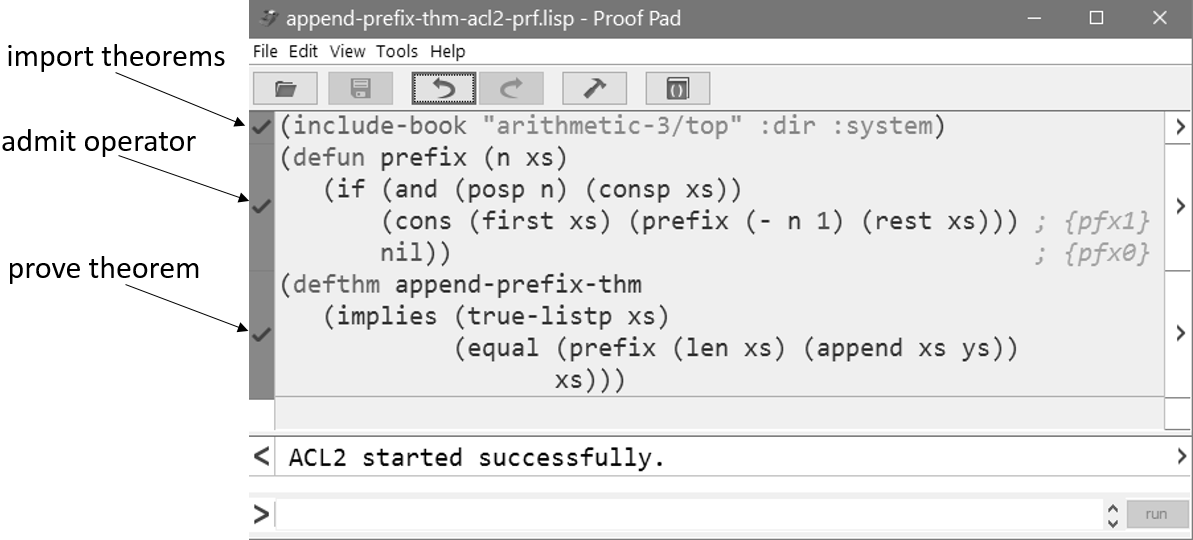
\includegraphics[scale=0.43]{images/append-prefix-thm-acl2-prf-bw.png}
\end{center}
\index{append!prefix theorem}\index{theorem!append-prefix}
\index{theorem, by name!\{append-prefix\}}
\caption{Append-Prefix Theorem: an Implication}
\label{fig:append-prefix-acl2-prf}
\end{figure}

Now we have a theorem that we believe is true
based on our pencil-and-paper proof.
The mechanized logic of ACL2
succeeds in proving this theorem, but, as was the case with
the append suffix theorem
(Figure~\ref{fig:append-suffix-acl2-prf}, page \pageref{fig:append-suffix-acl2-prf}),
it needs to cite some theorems of numeric algebra.
Figure~\ref{fig:append-prefix-acl2-prf} (page \pageref{fig:append-prefix-acl2-prf})
displays a Proof Pad session that imports those theorems,
defines the prefix operator, and then states and proves the theorem.
The figure indicates that ACL2
``admits'' the prefix operator when it encounters its definition.
This means that ACL2 allows the definition to join
the universe of entities that can participate in
the mechanized reasoning process.
Aside~\ref{reason-for-acl2-admit} (page \pageref{reason-for-acl2-admit})
explains what this entails.

\begin{aside}
In Figure~\ref{fig:append-prefix-acl2-prf}
there is a step that has the label ``admit operator''.
That is the terminology ACL2 uses for the process of accepting
an operator into its mechanized logic.
A domain in which operators may fail to terminate
calls for a more complex reasoning process than a domain that is
restricted to operators that are guaranteed to complete their
computation in a finite number of steps.
To give itself a better shot at succeeding in mechanized proofs,
ACL2 does not deal with operators with a potential for non-termination.
It admits operators to its domain of logic
only if it can verify termination in all cases.
Sometimes, coming up with an operator definition that makes
it possible for ACL2 prove termination is, by itself,
a major project, including importing theorems or coming up with new
theorems to facilitate the reasoning process.
Hardware and software with guaranteed properties is not easy to come by.
\index{admit, ACL2}\index{ACL2!admit}
\caption{ACL2 Must Prove That Operators Terminate}
\label{reason-for-acl2-admit}
\end{aside}

\begin{ExerciseList}

\Exercise Define the \{\emph{rep-len}\} theorem (page \pageref{rep-len}) in ACL2 notation,
and use Proof Pad to run it through the ACL2 mechanized logic.
(Hint: You will need to constrain the first operand of rep to the domain of natural numbers.)

\Exercise An exercise in Section~\ref{sec:append-prefix-suffix} required a pencil-and-paper
proof of the following proposition: $\forall xs.$((nthcdr (len \emph{xs}) $xs$) $=$ nil).
Define this theorem in ACL2 notation and get the mechanized logic to prove it.

\Exercise The formula (equal (prefix (len $xs$) $xs$) $xs$) is true with a certain
constraint on $xs$. Define an ACL2 theorem with this equation as its conclusion
and get the mechanized logic to prove it.

\end{ExerciseList}

\section{Helping Mechanized Logic Find Its Way}
\label{sec:lemmas}

The mechanized logic of ACL2 was able to carry out proofs of
the theorems of Section~\ref{sec:theorems-and-acl2-proofs} without assistance.
To prove the theorems in Section~\ref{sec:using-books-of-proven-theorems},
ACL2 needed to cite some proven theorems packaged in books
developed by experts.
These were carefully chosen examples to get started with
the mechanized proofs.
Usually, the process of using a mechanized logic requires
both proven theorems packaged in books
and specialized theorems chosen to match the
needs of a particular goal.
That is, to succeed in proving a complex property of
an operator defined in ACL2,
it is usually necessary to prove
some simpler properties that the mechanized
logic can cite in a proof of the more complex property.

\index{ACL2!helping}Choosing simpler properties that ACL2 can prove
and building, finally, to the more complex proof
calls for insight and creativity.
This is where your experience with pencil-and-paper proofs
come in handy.
You can plan a strategy by thinking of major steps
in a proof, stating those steps as separate theorems,
and proving them one by one to build up a body
of helpful theorems that the mechanized logic
can cite to move closer to the goal.

It may help to see an example of how this can work.
The Fibonacci numbers are a well-studied sequence that
scientists have used to study
patterns of development in leaves and flowers,
growth rates in animal populations,
and other natural phenomena.
The sequence can be defined inductively
with the Fibonacci equations
(Figure~\ref{fig:Fibonacci-axioms}, page \pageref{fig:Fibonacci-axioms}).

\begin{figure}
\begin{center}
\emph{Axioms \{Fibonacci\}}
\begin{tabular}{ll}
$f_0$ $=$ $0$                   & \{\emph{f0}\} \\
$f_1$ $=$ $1$                   & \{\emph{f1}\} \\
$f_{n+2}$ $=$ $f_{n+1} + f_{n}$ & \{\emph{f2}\} \\
\end{tabular}
\begin{Verbatim}
(defun fib(n) ; n-th Fibonacci number
  (if (posp (- n 1))                      ; n > 1
      (+ (fib(- n 1)) (fib(- n 2)))       ; {fib2}
      n))                                 ; {fib1}
\end{Verbatim}
\begin{tabular}{llllllllll}
\dots & (fib 2) & (fib 3) & (fib 4) & (fib 5) & \dots & (fib 10) & (fib 11) & (fib 12) & \dots \\
\dots & ~~~~~1  &  ~~~~2  &  ~~~~3  &  ~~~~5  & \dots &  ~~~~~55 &  ~~~~~89 & ~~~144   & \dots \\
\end{tabular}
\end{center}
\index{Fibonacci!numbers}\index{axiom!Fibonacci}
\index{operator, by name!fib, fib-fast (Fibonacci)}
\index{Fibonacci!operator}
\index{equation, by name!\{f0\}, \{f1\}, \{f2\}}
\index{equation, by name!\{fib1\}, \{fib2\}}
\index{axiom, by name!\{f0\}, \{f1\}, \{f2\}}
\caption{Fibonacci Numbers}
\label{fig:Fibonacci-axioms}
\end{figure}

The Fibonacci operator, fib, defined in ACL2
mirrors the algebraic equations.
It selects the inductive formula,
(fib$(n - 1)$) + (fib$(n - 2)$),
for an operand $n$ that is 2 or bigger
(that is, when $(n-1)$ is a positive, natural number).
For smaller operands, the ACL2 definition
observes that the corresponding Fibonacci number
is the same as the operand:
(fib 0) $=$ $f_0$ $=$ $0$ by axiom \{\emph{f0}\}
and (fib 1) $=$ $f_1$ $=$ $1$ by axiom \{\emph{f1}\}.

We can be confident that $\forall n.($(fib $n$) $=$ $f_n)$
because the ACL2 definition of fib is a direct
transliteration of the Fibonacci equations.
We can use the operator fib as a calculator
to compute some Fibonacci numbers.
This works well for small numbers,
but it turns out that there are
a huge number of
computational steps required to derive
(fib $n$) from the Fibonacci axioms when $n$ gets above a few dozen.
For example the computation of (fib 30) proceeds quickly,
but you will see a noticeable delay if ask ACL2 to compute (fib 40),
and you would have to wait a long time for (fib 50).

It's not to hard to see the reason for this.
The axioms calculate (fib $(n+2)$) by first calculating
(fib $(n+1)$), and then calculating (fib $n$), and finally
adding those two numbers together.
However many computational steps it takes to compute (fib $n$),
it will take at least a few more to compute (fib $(n+1)$).
So, there will be more than twice as many steps in the computation of (fib $(n+2)$)
as there are in the computation of (fib $n$).
That is, when $n$ increases by 2, the number of computational steps more than doubles.
If we let $c_n$ stand for the number of computational steps in the calculation
of (fib $n$), then our observation about doubling amounts to the
inductive relationship $c_{n+2} \geq 2c_n$.
We think you have had enough experience to prove (by induction of course)
that $\forall n.(c_{2n+1} \geq 2^n)$,
assuming it takes at least one computational step to compute (fib $1$).
That's what they call ``exponential growth''.\footnote{The term
``exponential growth'' is bandied about a lot, but mostly
in ways that do not match the standard mathematical meaning.
The most common usage is to describe something that
gets big fast, which is certainly true of exponential growth,
but is also true of quadratic growth.
Quadratic growth often gets passed off, informally, as exponential growth,
but it's not even close. If the number of computational steps
in computing (fib $n$) from the axioms grew quadratically instead of exponentially,
it would not take a lot longer to compute (fib 40) than it does to compute (fib 30).}
It is dramatic, to say the least. We estimate that it would take an hour to compute
(fib 50) on a typical laptop computer and upwards of a year to compute (fib 75).

The Fibonacci axioms comprise an
\index{Fibonacci!definition}inductive definition.
They conform to the three C's
(Figure~\ref{fig:inductive-def-keys}, page \pageref{fig:inductive-def-keys}),
so they guarantee delivery of a Fibonacci number
in a finite number of computational steps.
Unfortunately, in this case it turns out to be
a huge number of computational steps.
Fortunately, there are alternatives.

If a particular inductive definition leads to a long computation,
there may be another inductive definition that produces the same
results with less work,
and that is the case with Fibonacci numbers.
Figure~\ref{fig:gib-defun} (page \pageref{fig:gib-defun})
displays another definition that uses a method known as
\index{tail recursion}\index{definition!tail recursive}
``tail recursion''.\footnote{\index{recursive}``Recursive definition''
is the most commonly used term for what we call ``inductive definition''.
We don't say recursive because the term is often conflated
with an implementation method based on a data structure called a stack,
and we think fixating on computational detail obscures the meaning
of the definition.
We want you to think of inductive (aka recursive)
definitions as axiomatic equations that can be used to reason about the
operators they define. We leave it to the computer system
to determine how to carry out the computation.
Sometimes, as in the Fibonacci problem
where an inductive definition leads to inefficient computation,
we will look for more efficient alternatives,
but we will not relinquish our view of operator definitions
as axioms to support reasoning. If our programming language allowed
mutable variables, as most programming languages do, we would
delve into a stack-based view of recursion.
Since it doesn't, we won't.}
A tail recursion is a circular reference in an operator definition
that occurs at the
\index{top level, vs nested}\index{nested, vs top level}``top level'',
which means that it is not nested
inside a formula to produce an operand for
another operator. The operator ``op'' occurs at the top level
in the formula (op $x$), but is nested in the formula (+ (op $x$) 1).
Most computing systems, including ACL2,
implement tail recursions efficiently. Nested recursions are
more problematic. They don't always lead to inefficient computations,
but sometimes, as with Fibonacci numbers, they do.

\begin{figure}
\begin{center}
\begin{Verbatim}
(defun gib (n b a)  ; b = (fib(n-1)), a=(fib(n-2))
   (if (posp (- n 1))
       (gib (- n 1) (+ b a) b)            ; {gib2}
       (if (= n 1)
           b                              ; {gib1}
           a)))                           ; {gib0}
(defun fib-fast (n) ; (fib-fast n)=(fib n)
   (gib n 1 0))     ; (fib 1)=1, (fib 0)=0
\end{Verbatim}
\end{center}
\seeonlyindex{fib, fib-fast}{operator}\index{Fibonacci!fast}\index{Fibonacci!operator}
\index{operator, by name!fib, fib-fast (Fibonacci)}
\index{operator, by name!gib (iterative Fibonacci)}
\index{equation, by name!\{gib0\}, \{gib1\}, \{gib2\}}\index{gib (\emph{see also} operator)}
\caption{Fibonacci Numbers: Quick Delivery}
\label{fig:gib-defun}
\end{figure}

The downside is that \index{tail recursion!reasoning about}\index{reasoning!about tail recursion}reasoning
about tail recursive
definitions is often more challenging than reasoning about definitions
with nested recursion. One way to proceed, however,
is to define an operator both ways, prove that the two definitions
produce the same results, and then use the efficient definition
for computation and the inefficient one when it
simplifies the reasoning process.

If you look at the definition of fib-fast (Figure~\ref{fig:gib-defun})
closely, we think you will agree that, while it may seem plausible
that (gib $n$ $1$ $0$) is the $n^{th}$ Fibonacci number,
it isn't obvious.
Some reasoning is required.

Maybe ACL2 can take it on successfully.
We would like to know that $\forall n.($(fib-fast $n$) = (fib $n$)$)$.
The theorem in ACL2 terms can be stated as follows.
\begin{samepage}
\index{theorem, by name!\{fib=fib-fast\}}
\index{Fibonacci!fast}\index{theorem!Fibonacci fast}
\begin{center}
\begin{Verbatim}
(defthm fib=fib-fast ; (fib-fast n) = (fib n)
    (implies (natp n)
             (= (fib n) (fib-fast n))))
\end{Verbatim}
\end{center}
\end{samepage}

When ACL2 tries to prove this theorem it fails,
or at least it takes such a long time floundering that we interrupted it
to try something else.
We thought maybe it needed to know some theorems from numeric
algebra, so we imported the arithmetic-3/top book, as usual,
but that didn't help. It still sat there spinning,
so we interrupted it again.

We guessed that it might be having trouble coming up with an effective
induction hypothesis, so we decided to ask it to prove that
the gib operator satisfies the basic Fibonacci axioms.
This is, to prove that the $n^{th}$ value of gib is
the sum of the previous two values (as in axiom \{\emph{f2}\}).
In ACL2 that theorem can be stated as follows.
\begin{samepage}
\index{gib (\emph{see also} operator)}
\index{theorem!gib lemmas (base, inductive)}
\index{gib (\emph{see also} operator)!lemmas (base, inductive)}
\begin{center}
\begin{Verbatim}
(defthm gib-inductive-equation ; a la {fib2}
    (implies (posp (- n 1))              ; n > 1
             (= (gib n b a)              ; n-th
                (+ (gib (- n 1) b a)     ; (n-1)th
                   (gib (- n 2) b a))))) ; (n-2)th
\end{Verbatim}
\end{center}
\end{samepage}

It fails quickly this time and reports that it was not able
to find an induction scheme that worked.
So, our attempt to help ACL2 along didn't work, exactly,
but at least ACL2 could determine quickly that
things were not going well.
Next, we decided that ACL2 might need help with the
base case as well as the inductive case, so we
stated a base case for the gib operator as an ACL2 theorem.

\begin{samepage}
\index{theorem!gib lemmas (base, inductive)}\index{gib (\emph{see also} operator)!lemmas (base, inductive)}
\begin{center}
\begin{Verbatim}
(defthm gib-base-equation ; a la {fib1}
    (= (gib 1 b a) b))
\end{Verbatim}
\end{center}
\end{samepage}

This idea worked. ACL2 was able to prove the gib-base-equation
and the gib-inductive-equation, and then, finally,
use them to prove that $\forall n.($(fib-fast $n$) = (fib $n$)$)$,
in the form defined in the fib=fib-fast theorem.
Figure~\ref{fig:fib-gib-thm} (page \pageref{fig:fib-gib-thm})
displays the Proof Pad session with the check-marks
indicating completed proofs by the mechanized logic of ACL2.

\begin{figure}
\begin{center}
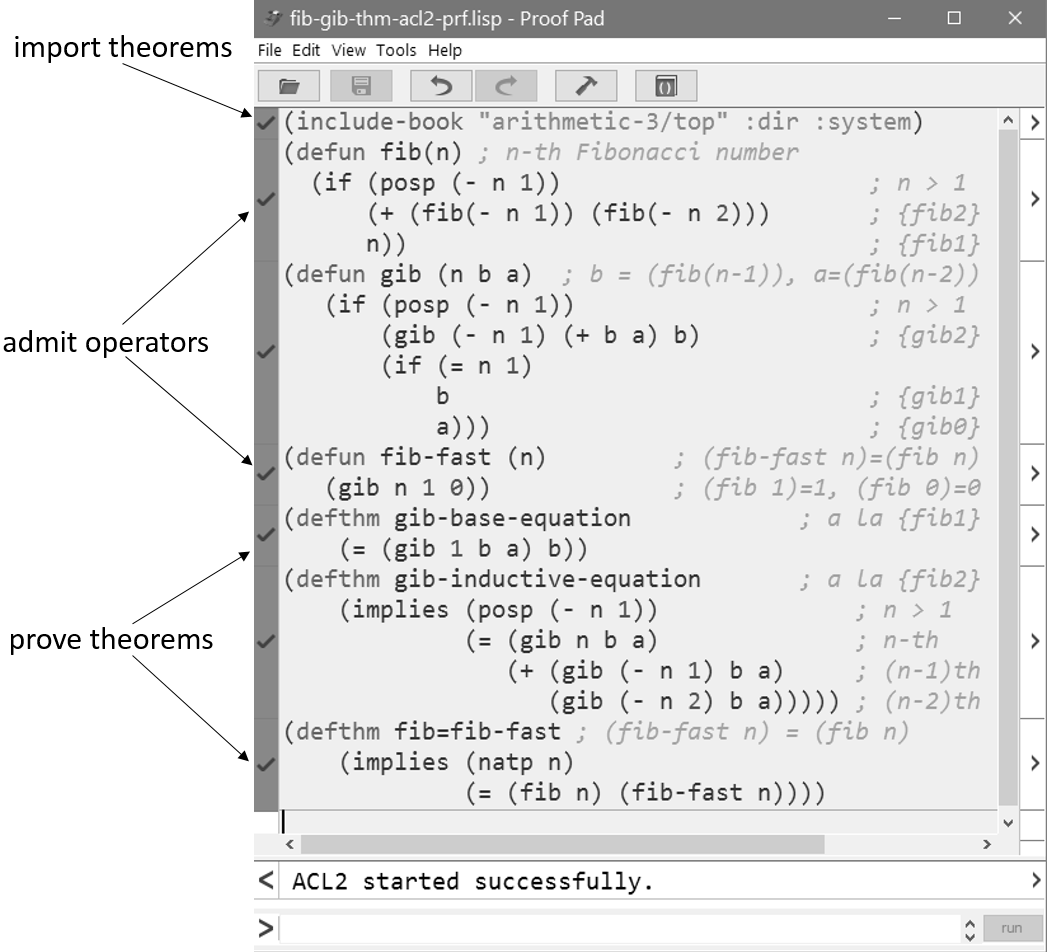
\includegraphics[scale=0.5]{images/fib-gib-thm-acl2-prf.png}
\end{center}
\caption{Fast Fibonacci Delivers Fibonacci Numbers}
\label{fig:fib-gib-thm}
\end{figure}

Try out the fib-fast operator in a Proof Pad session.
The Fibonacci number (fib-fast $n$) seems to appear
instantaneously, even for large values of $n$.

\begin{ExerciseList}

\Exercise Assume that $c_1 = 1$ and $c_{n+2} = 2c_n$.
Prove that $\forall n.(c_{2n+1} = 2^n)$.\\
\emph{Hint}: Define $x_n = c_{2n+1}$.
First, verify that $x_{n+1} = 2x_n$.
Then, use mathematical induction to prove that $x_n = 2^n$,
and translate this formula for $x_n$
to a formula for $c_{2n+1}$.\\
\index{exponents, law of}\emph{Note}: $2^0 = 1$, $\forall n.(2^{n+1} = 2 \times 2^n)$ \{\emph{Law of Exponents}\}

\end{ExerciseList}

\section{Proof Automation and Things That Can't Be Done}
\label{sec:halting-problem}

By now you've had some experience constructing proofs, and if you're like most people,
it has been tough going most of the time.
It's rarely easy to figure out how to prove a theorem,
and it's often extraordinarily difficult.
How is it, then, that a mechanized logic like ACL2 can succeed at such a difficult task?
How does ACL2 prove theorems?

First of all, it doesn't, most of the time.
Our examples have been carefully constructed in a way that
led to a successful proof by ACL2.
If you try, on your own, to propose theorems
and present them to ACL2 for proof, you will find that it can be
extremely difficult to get ACL2 succeed, even with a lot of help.
Often, you will need to sketch a proof yourself,
then give ACL2 a sequence of smaller theorems
that it can prove, one by one, building up to
the theorem that was your goal in the first place,
with plenty of roadblocks and changes in strategy along the way.

Even when all ACL2 has to do is fill in a few gaps,
we find it remarkable that ACL2 can succeed in proving theorems.
And, it \emph{is} remarkable.
When researchers began trying to automate parts
of the theorem proving process, it was many years
before really effective tools began to emerge.
Now, mechanized logics play a role in
the verification of important properties of digital circuits and
software, not only in research labs,
but also in engineering projects with deadlines and product cycles.
It's not just ACL2. There are many systems of mechanized logic that
have been developed over the past half-century or so,
by distinguished researchers in the USA, the UK, France, Sweden, and elsewhere.

\begin{aside}
\begin{itemize}
\item ACL2 (and precursor nqthm): J Moore, Robert Boyer, and Matt Kaufmann, Univ of Texas, with a long history starting at the Univ of Edinburgh and continuing at Xerox PARC and SRI
\item LCF, HOL, Isabelle: Robin Milner, Mike Gordon, Lawrence Paulson, Stanford Univ, Cambridge Univ, Univ of Edinburgh
\item Coq: Thierry Coquand, G\'erard Huet, INRIA, Univ of Gothenburg
\item PVS: Sam Owre, Natarajan Shankar, John Rushby, SRI
\item Agda: Ulf Norell, Chalmers Univ
\item LF: Robert Harper, Furio Honsell, Gordon Plotkin, Carnegie Mellon Univ, Univ of Udine, Univ of Edinburgh
\item Twelf: Frank Pfenning, Carsten Sch\"urmann, Carnegie Mellon Univ, Univ of Copenhagen
\end{itemize}
\index{logic!mechanized}
\index{Twelf}\index{Pfenning!Frank}\index{Sch\"urmann, Carsten}
\index{LF}\index{Harper, Robert}\index{Honsell, Furio}\index{Plotkin, Gordon}
\index{Agda}\index{Norell, Ulf}
\index{PVS}\index{Owre, sam}\index{Natarajan, Shankar}\index{Rushby, John}
\index{Coq}\index{Coquand, Thierry}\index{Huet, G\'erard}
\index{LCF}\index{HOL}\index{Isabelle}\index{Milner, Robert}\index{Gordon, Mike}\index{Paulson, Lawrence}
\index{ACL2}\index{Moore, J Strother}\index{Boyer, Robert}\index{Kaufmann, Matt}
\caption{Mechanized Logics: Fifty Years of R\&D, Mostly R}
\label{mechanized-logic-history}
\end{aside}

Proofs are not only hard.
They are sometimes impossible, as G\"odel famously proved in 1931
to the great surprise of many mathematicians of the day.
In the same vein there are things computers cannot do.
A well known example is the \index{halting problem} \emph{halting problem}, which
was proved to be outside the realm of computation
by \index{Turing, Alan}Alan Turing in 1936
and, independently, by \index{Church, Alonzo}Alonzo Church.
There were no computers at the time,
but there were mathematical models of computation
that are used, still today, to study the capabilities of computers.

A program solving the
\index{uncomputable}\index{halting problem}halting problem would be able to determine,
given a computer program, whether or not the program would terminate
in a finite amount of time, given a particular input.
There are programs that can solve the halting problem for
a limited set of programs,
but no program can solve the halting problem for all programs.
Proving that the halting problem is unsolvable is tricky,
but the basic idea of the proof is not too difficult to follow, and
it provides an example of reasoning that,
in a perverse sense, fits into a discussion of mechanized logic,
since it exhibits something that neither computers
nor people can do. There are many such things, as a search
using the key "uncomputable" shows.

To be specific, the following discussion of the halting problem
limits itself to a single programming language, but
that restriction turns out to be immaterial.\footnote{The
halting problem cannot be solved
for any ``general purpose'' \index{programming language}programming language,
by which we mean a \index{Turing complete}Turing complete language,
which itself calls for a long explanation even
before arriving at a discussion of how Turing completeness
interacts with the halting problem.
You can track that down, if you're interested.
All widely-used programming languages,
including \index{ACL2}ACL2, \index{Java}Java, and \index{C++}C++ for example, are \index{Turing complete}Turing complete.
We leave it at that.}
Because the discussion the halting problem is clumsy in ACL2,
we'll present the ideas in terms of a different
language that has the same syntax
and similar interpretation. That language is Lisp.
For the purposes of this discussion,
you can think of Lisp as ACL2 with the added feature
of allowing operators to act as operands.
That is, a formula invoking an operator can supply
another operator as input.
Most programming languages allow this.
ACL2 doesn't because the extra facility
interferes with some of the strategies that ACL2 uses
to mechanize the process of proving theorems.

The discussion will include some logic formulas with
quantification,
so we need to specify the universe of discourse
(page \pageref{def-universe-of-discourse}).
When the bound variable
in the formula is $h$, the universe of discourse
is the set of operators that have
two operands and can be defined in Lisp:
(defun $h$ ($f$ $x$) \dots \emph{Lisp formula} \dots ).
When the bound variable is $f$,
the universe of discourse is  set of operators
that have one operand and can be defined in Lisp:
(defun $f$ ($x$) \dots \emph{Lisp formula} \dots ).\footnote{The
restriction to one operand simplifies the presentation,
but is not really a restriction because the operand could
be a list containing any number of values.}
When the bound variable is $x$, the universe of discourse
is the set of values that Lisp operators can deliver.

We define a predicate, $H$, that tells us whether or not
a particular formula in Lisp represents a computation that terminates,
that is, a computation that would be completed in a finite amount of time.
$H$ is not a Lisp operator and does not, itself,
represent a computation. It is a mathematical entity
outside the realm of computation that gives us a way
to use symbols and formulas to talk about
whether or not a computation terminates.

The definition of the predicate $H$ uses the Lisp
formula ($f$ $x$) to designate a computation that may
or may not be completed in a finite amount of time.
Since $H$ is a logic predicate, not a computation,
it has a value whether or not the formula ($f$ $x$) terminates.
\begin{quote}
\index{predicate, by name!H (termination)}\index{termination predicate (H)}
\label{def:predicate-H}
\emph{Definition of predicate} $H$\\
\hspace*{3mm}$H(f, x) = False$, if ($f$ $x$) does not terminate\\
\hspace*{3mm}$H(f, x) = True$, if ($f$ $x$) terminates
\end{quote}

The theorem that Turing and Church proved is that
no operator $h$ can be defined in Lisp
that accepts a Lisp operator $f$ as its
first operand and a Lisp value $x$ as its second operand
such that, regardless of the definition of the operator $f$,
($h$ $f$ $x$) = 0 if the computation ($f$ $x$) terminates, and
($h$ $f$ $x$) = 1 if ($f$ $x$) does not terminate.
This means not just that it would be hard to define the operator $h$.
It means that nobody can define $h$ with any amount of effort or cleverness.
There is no such definition.
There are some things that cannot be done, and this is one of them.

\label{church-turing-hypothesis}
\index{Church-Turing hypothesis}\index{Turing-Church hypothesis}\index{hypothesis!Church-Turing}
A conjecture of Church and Turing
concerning the effectiveness of general-purpose programming languages
asserts that for any computation that can be carried out, there is a program
that can be written in Lisp (or any other general-purpose programming language)
that specifies a way to carry out the computation.
If one believes Church-Turing conjecture, and most computer scientists do,
then the theorem that Church and Turing proved about the prospects of
automating the prediction of program termination
says that no program can be written that solves the halting problem.
Neither Turing nor Church stated the theorem in terms of Lisp.
Turing used a model of computation known as the Turing machine, and
Church used the lambda calculus, another model of computation.
Both models are still widely studied in computer science theory.
The programming language Lisp
was based on the lambda calculus, so the two are closely related.

We express the \index{halting problem}halting problem theorem as a logic formula that we will prove
using natural deduction (Section \ref{sec:deduction}).
The theorem has no hypotheses.
\begin{quote}
\index{theorem!halting problem}\index{theorem, by name!\{halting problem\}}
Theorem \{halting problem\}:\\
$\vdash$ $\neg(\exists h. \forall f. \forall x.
((H(f, x) \rightarrow ($($h$ $f$ $x$) $ = 1)) \wedge ((\neg H(f, x)) \rightarrow ($($h$ $f$ $x$) $= 0))))$
\end{quote}

There are two Lisp formulas embedded in
the logic formula of the theorem, both the same:
($h$ $f$ $x$).
Those formulas invoke an operator $h$, which is defined in Lisp because that is the universe
of discourse for $h$, the bound variable in the $\exists$ quantification.
The logic formula then compares the value that
the formula ($h$ $f$ $x$) represents to a natural number.

To make the proof more compact and, we hope, more readable,
we will use $E$ as an abbreviation for the
long $\exists$ formula whose negation is the conclusion of the theorem.
\begin{quote}
$E$ $\equiv$ $\exists h. \forall f. \forall x.
((H(f, x) \rightarrow ($($h$ $f$ $x$) $ = 1)) \wedge ((\neg H(f, x)) \rightarrow ($($h$ $f$ $x$) $= 0)))$
\end{quote}

With the abbreviation, the \{halting problem\} theorem is: $\vdash$ $\neg E$.
Figure~\ref{fig:halting-proof-strategy} (page \pageref{fig:halting-proof-strategy})
displays the proof, which uses the natural deduction formalism.
It cites a theorem we already proved (Theorem \{$\neg \neg$ forward\}) and
a Theorem \{paradox\}, which we will prove
after showing how our goal, the \{halting problem\} theorem,
can be derived from it.
To clarify the derivation, we need to state the \{paradox\} theorem,
which we will prove later.
\begin{quote}
\index{theorem!paradox}\index{theorem, by name!\{paradox\}}
\index{paradox, halting problem}\index{halting problem}
Theorem \{paradox\}: $E$ $\vdash$ $False$
\end{quote}

In addition to citing the \{paradox\} theorem,
the proof of the \{halting problem\} theorem
cites the \{reductio ad absurdum\} inference rule
(Figure~\ref{fig-02-deduction-rules}, page \pageref{fig-02-deduction-rules}),
so our proof of the \{halting problem\} theorem is a proof by contradiction.
It begins by assuming the negation of the formula in its conclusion.
The assumption, as always, stands in lieu of a proof.
As it happens, the assumption is discharged later in the proof,
leaving the \{halting problem\} theorem with no hypotheses,
as it is stated.

\begin{figure}
Theorem \{halting problem\}: $\vdash$ $\neg E$ ~~~~~~~~\emph{Note: This theorem has no hypotheses.}\\
proof~~~~(\emph{Note}: $E$ $\equiv$ $\exists h. \forall f. \forall x.
((H(f, x) \rightarrow ($($h$ $f$ $x$) $ = 1)) \wedge ((\neg H(f, x)) \rightarrow ($($h$ $f$ $x$) $= 0)))$)
\begin{center}
\begin{tabular}{ll}
Assume $(\neg(\neg E))$                       &\emph{discharged later; E abbreviates long $\exists$ formula}\\
------------------------\{$\neg \neg$ forward\} &\emph{proved in Figure~\ref{fig:dbl-neg-fwd} (page \pageref{fig:dbl-neg-fwd})}\\
~~~~~~~~~~~~$E$                               &\\
------------------------\{paradox\}           &\emph{proved in Figure~\ref{fig:proof-paradox-thm} (page \pageref{fig:proof-paradox-thm})}\\
~~~~~~~~$False$                               &\\
------------------------\{$\rightarrow$ introduction\} &\emph{assumed} $(\neg(\neg E))$\emph{, proved} $False$\emph{,}\\
~~$(\neg(\neg E)) \rightarrow False$          &~~~~\emph{conclude} $(\neg(\neg E)) \rightarrow False$\\
Discharge $(\neg(\neg E))$                    &\emph{eliminates} $(\neg(\neg E))$\emph{, leaving no hypotheses}\\
------------------------\{reductio ad absurdum\}&\emph{Figure~\ref{fig-02-deduction-rules} (page \pageref{fig-02-deduction-rules})}\\
~~~~~~~~~~~$\neg E$                           &\emph{no program solves halting prob for all programs}\\
\end{tabular}
\end{center}
\index{halting problem}\index{theorem!halting problem}
\index{theorem, by name!\{halting problem\}}
\caption{Theorem \{halting problem\}: a proof by contradiction}
\label{fig:halting-proof-strategy}
\end{figure}

We are not quite ready to tackle the \{paradox\} theorem.
The proof will be easier to follow if we break it into parts,
then connect the parts in the final analysis.

Recall that $E$, the hypothesis of the \{paradox\} theorem,
is a $\exists$ formula.
Since $E$ is a hypothesis of the \{paradox\} theorem,
we will assume at the beginning of the proof
the \{paradox\} theorem that $E$ is true.
$E$ asserts that there is at least one definition of
an operator $h$ that provides a universal, computational solution
to the halting problem.
Since there is at least one such operator,
let's assume someone has handed us a
definition of the operator, and that the operator has the name h:
(defun h (f x)  \dots \emph{Lisp formula} \dots ).

We don't know the definition of h, but the formula $E$
tells us some of its properties.
In particular, $E$ says that for any operator $f$ and any value $x$,
the formula (h $f$ $x$) = 0 if $H(f, x)$ is $False$ and
(h $f$ $x$) = 1 if $H(f,x)$ is $True$.
We specify those properties in the following two theorems.
\begin{quote}
\index{theorem, by name!\{hF\}}\index{theorem, by name!\{hT\}}
Theorem \{hF\}: $E$ $\vdash$ $\forall f.\forall x.(\neg H(f, x))$ $\rightarrow$ (h $f$ $x$) $= 0$\\
Theorem \{hT\}: $E$ $\vdash$ $\forall f.\forall x.H(f, x)$      $\rightarrow$ (h $f$ $x$) $= 1$
\end{quote}

Since h is a Lisp operator, we can refer to it in the definition of
another Lisp operator.
Figure~\ref{fig:paradox-op-defun} (page \pageref{fig:paradox-op-defun})
defines the operator p.
It invokes h to decide whether to deliver the value 0 or
the computation represented by an invocation of an operator called ``loop'',
which is also defined in
Figure~\ref{fig:paradox-op-defun}.
The loop operator doesn't do anything.
Or, rather,
it does way too much by doing nothing over and over, forever.
We are going to take it on faith that (loop $x$) does not terminate,
regardless of the value of its operand $x$.
We think you can probably convince yourself of that,
so we assert that $\forall x.(H($loop, $x) = False)$.

\begin{figure}
\begin{center}
Axioms of p\\
\begin{tabular}{lll}
(p $x$) $= 0$          & if (h p $x$) $=  0$      &\{p0\}\\
(p $x$) $=$ (loop $x$) & if (h p $x$) $\neq 0$    &\{p1\}\\
\end{tabular}
\begin{Verbatim}
(defun loop (x)  ; a non-terminating computation
  (loop x))
(defun p (x)     ; definition derived from axioms of p
  (if (equal (h p x) 0)
      0
      (loop x)))
\end{Verbatim}
\end{center}
\index{loop}
\caption{Definitions of Operators p and loop}
\label{fig:paradox-op-defun}
\end{figure}

We can inquire about p using the predicate $H$.
In particular, we would like to know, given a value $x$,
whether $H($p, $x)=True$ or $H($p, $x)=False$.
It has to be one or the other because $H$ is a predicate.
Since p is an operator, $x$ is a value, and 1 is not 0,
the following theorems are special cases of
Theorem \{hF\} and Theorem \{hT\}.
\begin{quote}
\index{theorem, by name!\{pF\}}\index{theorem, by name!\{pT\}}
Theorem \{pF\}: $E$ $\vdash$ $(\neg H($p, $x))$ $\rightarrow$ (h p $x$) $= 0)$ \\
Theorem \{pT\}: $E$ $\vdash$ $H($p, $x)$ $\rightarrow$ $(\neg($(h p $x$) $= 0))$
\end{quote}

Now, let's reason from the definition of p (Figure~\ref{fig:paradox-op-defun}).
In the definition, we find that if (h p $x$) $= 0$, then (p $x$) $=0 $.
We also find that if (h p $x$) $\neq 0$, then (p $x$) represents
the computation (loop $x$). We will use the notation (p $x$) $=$ (loop $x$)
to indicate this relationship between (p $x$) and (loop $x$).\footnote{This
\label{caveat:equality-for-loop}
interpretation of the equation (p $x$) $=$ (loop $x$) conforms with
our usual practice of substituting the formula designated in the
definition of $f$ for an invocation ($f$ $x$).
That is, we interpret the substitution a new formula
in place of an old one with the same meaning as an equation
between the old formula and the new one.
It is an odd sort of equality in the case of (p $x$) $=$ (loop $x$)
because the formula (loop $x$) represents a computation, but not a value.
The loop operator at every stage delivers a new formula,
but never manages to produce a value.}
This reasoning verifies two more theorems:
\begin{quote}
Theorem \{h0\}: $\vdash$  (h p $x$) $=0$  $\rightarrow$ (p $x$) $= 0$    \\
Theorem \{h1\}: $\vdash$  $\neg($(h p $x$) $= 0)$ $\rightarrow$ (p $x$) $=$ (loop $x$)
\end{quote}

If we apply the definition of $H$ again (page \pageref{def:predicate-H})
and observe that (1)~(p $x$) $= 0$ implies that (p $x$) terminates and
(2)~(p $x$) $=$ (loop $x$) implies that (p $x$) does not terminate,
we get two more theorems:
\begin{quote}
Theorem \{p0\}: $\vdash$  (p $x$) $= 0$ $\rightarrow$ $H($p, $x)$ \\
Theorem \{p1\}: $\vdash$  (p $x$) $=$ (loop $x$) $\rightarrow$ $(\neg H($p, $x))$
\end{quote}

From the three theorems, \{pF\}, \{h0\}, and \{p0\},
we can derive Theorem \{H$+$\}, and
from the other three theorems, \{pT\}, \{h1\}, and \{p1\},
we can derive
\index{halting problem}Theorem \{H$-$\}.
\begin{quote}
Theorem \{H$+$\}: $E$ $\vdash$ $(\neg H($p, $x))\rightarrow H($p, $x)$ \\
Theorem \{H$-$\}: $E$ $\vdash$ $H($p, $x) \rightarrow(\neg H($p, $x))$
\end{quote}

Figure~\ref{fig:hminus-thm-proof} (page \pageref{fig:hminus-thm-proof}) displays
a proof of Theorem \{H$-$\}.
The proof of Theorem \{H$+$\} is similar, and working through it would be
a good way to get a solid understanding the proof in Figure~\ref{fig:hminus-thm-proof}.

\begin{figure}
Theorem \{H$-$\}: $E$ $\vdash$ $H($p, $x) \rightarrow(\neg H($p, $x))$~\\
proof
\begin{center}
\begin{tabular}{ll}
~~~~~~~~~~Assume $E$                                &\emph{hypothesis of theorem}\\
-------------------------------------------\{pT\}   &\\
$H($p, $x)$ $\rightarrow$ $(\neg($(h p $x) = 0))$   &\\
 - - - - - - - - - - - - - - - - - - - - - - - - - -&\emph{separates 2 proofs req'd to cite} \{$\rightarrow$ chain\} \emph{thm}\\
                                                    &\emph{no hypotheses required}\\
-------------------------------------------\{h1\}   &~~~~~~\emph{for Theorem} \{h1\}\\
$\neg($(h p $x)=0)$ $\rightarrow$ (p $x$) $=$ (loop $x$)&\\
-------------------------------------------\{$\rightarrow$ chain\} &\{$\rightarrow$ chain\} \emph{thm (Figure~\ref{fig:impchain-proof}, page \pageref{fig:impchain-proof})}\\
~~~$H($p, $x)$ $\rightarrow$ (p $x$) $=$ (loop $x$) &\\
 - - - - - - - - - - - - - - - - - - - - - - - - - -&\emph{separates 2 proofs req'd to cite} \{$\rightarrow$ chain\} \emph{thm}\\
                                                    &\emph{no hypotheses required}\\
-------------------------------------------\{p1\}   &~~~~~~\emph{for Theorem} \{p1\}\\
~~(p $x$) $=$ (loop $x$) $\rightarrow$ $(\neg H($p, $x))$ &\\
-------------------------------------------\{$\rightarrow$ chain\} &\emph{another citation of} \{$\rightarrow$ chain\} \emph{thm}\\
~~~~~~$H($p, $x)$ $\rightarrow$ $(\neg H($p, $x))$  &\\
\end{tabular}

\end{center}
\index{theorem, by name!\{H$-$\}}
\caption{Proof of Theorem \{H$-$\}}
\label{fig:hminus-thm-proof}
\end{figure}

The \{contradiction\} equation (page \pageref{boolean-contradiction}),
together with the \{double negation\} equation
(Figure~\ref{fig-02-grammar}, page \pageref{fig-02-grammar}),
prove that
$((\neg H($p, $x)$ $\rightarrow$ $H($p, $x)) = H($p, $x)$
and
$(H($p, $x)$ $\rightarrow$ $(\neg H($p, $x)))$ = $(\neg H($p, $x))$.


So, we can rewrite the \{H$+$\} and \{H$-$\} theorems as follows.
\begin{quote}
\label{thm:HplusHminus}
\index{theorem, by name!\{H$-$\}}\index{theorem, by name!\{H$+$\}}
Theorem \{H$+$ version 2\}: $E$ $\vdash$ $H($p, $x)$ \\
Theorem \{H$-$ version 2\}: $E$ $\vdash$ $\neg H($p, $x)$
\end{quote}

Now, at last, we're ready to take on
the proof of Theorem \{paradox\}.
It derives $False$ from the contradiction that is apparent
in the \{H$+$\} and \{H$-$\} theorems.
Figure~\ref{fig:proof-paradox-thm} (page \pageref{fig:proof-paradox-thm})
displays this final step in our proof
of the theorem of Turing and Church,
confirming that the halting problem cannot be solved.

\begin{figure}
Theorem \{paradox\}: $E$ $\vdash$ $False$\\
proof
\begin{center}
\begin{tabular}{ll}
~~~~~Assume $E$                                 &\emph{hypothesis of theorem}\\
------------------------\{H$+$ version 2\}      &\emph{proof of} \{H$+$\} \emph{left as exercise}\\
~~~~~~~~~~$H($p, $x)$                           &\\
 - - - - - - - - - - - - - - - - - - - - - - - -&\emph{separates 2 proofs req'd to cite} \{$\wedge$ complement\} \emph{thm}\\
~~~~~Assume $E$                                 &\emph{hypothesis of theorem}\\
------------------------\{H$-$ version 2\}      &\emph{\{H$-$\} proved in Figure~\ref{fig:hminus-thm-proof} (page \pageref{fig:hminus-thm-proof})}\\
~~~~~~~~$\neg H($p, $x)$                        &\\
------------------------\{$\wedge$ complement\} &\emph{see Figure~\ref{thm:and-complement}, page \pageref{thm:and-complement}}\\
~~~~~~~~~~~$False$                              &\\
\end{tabular}
\end{center}
\index{theorem!paradox}\index{theorem, by name!\{paradox\}}
\index{theorem, by name!\{halting problem\}}
\index{halting problem}
\caption{Theorem \{halting problem\}: a proof by contradiction}
\label{fig:proof-paradox-thm}
\end{figure}

\begin{ExerciseList}
\Exercise Prove Theorem \{H$+$\} (page \pageref{thm:HplusHminus}).

\Exercise \label{ex:loop-loop}
Suppose $x$ is a suitable operand for the operator loop
(Figure~\ref{fig:paradox-op-defun}, page \pageref{fig:paradox-op-defun}).
Prove that the formula
\index{loop}
(loop $x$) represents
the same computation as the formula (loop (loop $x$)).

\Exercise \label{ex:loop-n}
Suppose $f$ is an ACL2 operator, $x$ is an ACL2 value,
and $n$ is a natural number.
The following equations define the notation ($f^n$ $x$).
\index{iteration}
\index{equation, by name!\{iter0\}, \{iter1\}}
\begin{center}
\begin{tabular}{ll}
($f^0$ $x$) $=$ $x$                    &\{iter0\} \\
($f^{n+1}$ $x$) $=$ ($f$ ($f^n$ $x$))  &\{iter1\} \\
\end{tabular}
Example: ($f^3$ $x$) $=$ ($f$ ($f$ ($f$ $x$)))
\end{center}
Interpreting the relationship between (loop $x$) and (loop (loop $x$))
stated in Exercise~\ref{ex:loop-loop}
as an equation (see footnote, page \pageref{caveat:equality-for-loop}),
use mathematical induction to verify the following formula.
\begin{quote}
$\forall n.\forall x.($(loop $x$) $=$ (loop$^{n+1}$ $x$)$)$
\end{quote}

\Exercise \label{ex:f-n}
Assume that $f$ is an operator and $x$ is an appropriate operand for $f$.
Assuming that it takes at least one computational step to compute ($f$ $x$).
Prove by induction that it takes at least $n$ computational steps
to compute ($f^n$ $x$), where ($f^n$ $x$) satisfies the axioms
\{iter0\} and \{iter1\} in Exercise~\ref{ex:loop-n}.

\Exercise
Suppose $x$ is a suitable operand for the operator loop
(Figure~\ref{fig:paradox-op-defun}, page \pageref{fig:paradox-op-defun}).
Let $T$ stand for the number of computation steps required to
compute (loop $x$).
Using the definitions and theorems of Exercise~\ref{ex:loop-loop},
Exercise~\ref{ex:loop-n}, and Exercise~\ref{ex:f-n},
prove that $(\forall n.(T > n))$, where the universe of
discourse of $\forall n$ is the natural numbers.

\end{ExerciseList}

\todo{
DONE 21Sep2017
Put labels on sections, at least in Ch2.tex
label for nat deduc section: \section{Deduction} \label{sec:deduction}

DONE 21Sep2017
Add label to first exercise, nat deduc section:
\Exercise
\label{thm:and-complement}
Use natural deduction to prove
Theorem \{$\wedge$ complement\}: $a$, $\neg a$ $\vdash$ $False$

DONE before 21Sep2017
Add label to natp explanation in ch3.tex:
\label{natp-op}
The value of the formula ``(natp $x$)'' is true

DONE 21Sep2017
Insert absurd-1 and absurd-2 equations just before absurdity equation in table in ch2.tex
$((x \rightarrow y) \wedge (x \rightarrow z)) = (x \rightarrow (y \wedge z))$ & \{$\wedge$ implication\} \label{and-implication} \\
$(x \rightarrow (\neg x)) = (\neg x)$                                & \{absurd 1\}               \label{absurd-1} \\
$((\neg x) \rightarrow x) = (\neg x)$                                & \{absurd 2\}               \label{absurd-2} \\
%% YIKES! {absurd 2} is false, and {absurd 1} is identical to the {contradiction} equation
%% PULLED BOTH, FIXED "Some Boolean Theorems" figure and other reference
%% THE ONLY OTHER CITATION WAS IN THE HALTING PROBLEM PROOF, AND THAT CITATION WAS WRONG
%% SO ALL THAT WAS NEEDED WAS TO PULL IT THERE, TOO
$((x \rightarrow y) \wedge (x \rightarrow (\neg y))) = (\neg x)$     & \{absurdity\}              \label{absurdity} \\
}
%%\end{comment}
%% All references to Dracula taken out (30Aug2017 - rlp)
%% I think we should use Proof Pad for all doublecheck and other interface-to-ACL2 issues.
%% We can explain in an aside, when we first mention Proof Pad,
%%    that ACL2s and emacs are other interfaces,
%%    that ACL2s has its own, extensive, random-test facility,
%%    that it is perfectly reasonable for students to use another interface to ACL2,
%%    that if they use another interface, they will need to interpret our doublecheck examples in, say, ACL2 fashion.

%%% Local Variables:
%%% mode: latex
%%% TeX-master: "book"
%%% End:
